\documentclass{article}
\usepackage[utf8]{inputenc}
\usepackage{authblk}
\usepackage{graphicx}
\usepackage{multirow}
\usepackage{natbib}
\usepackage[table,xcdraw]{xcolor}
\usepackage{hyperref}
\usepackage{float}
\usepackage[T1]{fontenc}

\interlinepenalty=1000

\newcommand\coordinator[1]{\begin{flushleft}\small\textit{#1}\end{flushleft}}

\title{Proceedings of the OHBM Hackathon 2023}
\date{}

\author[1]{Yu-Fang Yang}
\author[2]{Anibal Sólon Heinsfeld}
\author[32]{Andrea Gondová}
\author[6]{Bruno Hebling Vieira}
\author[5]{Qing (Vincent) Wang}
\author[3,4]{Sina Mansour L.}
\author[7]{Xinhui Li}
\author[33]{Beau Haugen}
\author[8]{Alessandra Pizzuti}
\author[0]{Andrew Zalesky}
\author[9]{Annie G. Bryant}
\author[0]{Arshitha Basavaraj}
\author[0]{B.T. Thomas Yeo}
\author[10]{Bernd Taschler}
\author[11]{Boris Clénet}
\author[0]{Caio Seguin}
\author[11]{Camille Maumet}
\author[12]{Céline Provins}
\author[0]{Darin Erat Sleiter}
\author[11]{Élodie Germani}
\author[12]{Elodie Savary}
\author[0]{Fernanda Ponce}
\author[0]{Florian Rupprecht}
\author[0]{James Kent}
\author[13]{Jason Kai}
\author[14,15]{Jayson Jeganathan}
\author[16]{Jeff Mentch}
\author[17]{Ju-Chi Yu}
\author[0]{Kendra Oudyk}
\author[8]{Kenshu Koiso}
\author[18]{Kevin R. Sitek}
\author[0]{Lea Waller}
\author[0]{Maria Di Biase}
\author[19]{Mary Miedema}
\author[20]{Matthieu Joulot}
\author[21]{Max Korbmacher}
\author[22]{Natasha Clarke}
\author[0]{Niousha Dehestani}
\author[23]{Omer Faruk Gulban}
\author[0]{Oscar Esteban}
\author[24]{Paul A. Taylor}
\author[0]{Reinder Vos de Wael}
\author[0]{Remi Gau}
\author[25]{Sarah Goodale}
\author[26]{Simon R. Steinkamp}
\author[28,29,30]{Stefano Moia}
\author[31]{Thomas Maullin-Sapey}
\author[0]{Tristan Kuehn}
\author[0]{Yaroslav Halchenko}
\author[0]{Yifan Yu}
\author[22]{Marie-Eve Picard}
\author[0]{François Lespinasse}

\affil[1]{Division of Experimental Psychology and Neuropsychology, Department of Education and Psychology, Freie Universität Berlin}
\affil[2]{Department of Psychology, Center for Perceptual Systems, The University of Texas at Austin, Austin, Texas, United States}
\affil[3]{Centre for Sleep and Cognition & Centre for Translational Magnetic Resonance Research, Yong Loo Lin School of Medicine, National University of Singapore, Singapore}
\affil[4]{Department of Psychiatry, The University of Melbourne and Melbourne Health, Victoria, Australia}
\affil[5]{Shanghai Mental Health Center, School of Medicine, Shanghai Jiao Tong University, Shanghai, China}
\affil[6]{Department of Psychology, Faculty of Arts and Social Science, University of Zurich, Zurich, Switzerland}
\affil[7]{School of Electrical and Computer Engineering, Georgia Institute of Technology, Atlanta, Georgia, United States}
\affil[8]{Department of Cognitive Neuroscience, Faculty of Psychology and Neuroscience, Maastricht University, Maastricht, The Netherlands}
\affil[9]{School of Physics, The University of Sydney, Sydney, Australia}
\affil[10]{Big Data Institute, University of Oxford, United Kingdom}
\affil[11]{Univ Rennes, Inria, CNRS, Inserm, Rennes, France}
\affil[12]{Department of Radiology, Lausanne University Hospital and University of Lausanne, Lausanne, Switzerland}
\affil[13]{Robarts Research Institute, Western University, London, Canada}
\affil[14]{School of Psychological Sciences, College of Engineering, Science and Environment, University of Newcastle, Newcastle, Australia}
\affil[15]{Hunter Medical Research Institute, Newcastle, Australia}
\affil[16]{Speech and Hearing Bioscience and Technology, Harvard University, Cambridge, United States}
\affil[17]{Campbell Family Mental Health Research Institute, Centre for Addiction and Mental Health, Toronto, Canada}
\affil[18]{Northwestern University, Evanston, United States}
\affil[19]{Department of Bioengineering, McGill University, Montreal, Canada}
\affil[20]{Paris Brain Institute, Paris, France}
\affil[21]{Department of Radiography, Faculty of Health and Social Sciences, Western Norway University of Applied Sciences, Bergen, Norway}
\affil[22]{Centre de recherche de l'Institut universitaire de gériatrie de Montréal, Montréal, Canada}
\affil[23]{Brain Innovation, Maastricht, The Netherlands}
\affil[24]{National Institutes of Health, Bethesda, United States}
\affil[25]{Department of Biomedical Engineering, Vanderbilt University, Nashville, United States}
\affil[26]{Danish Research Centre for Magnetic Resonance, Department of Radiology and Nuclear Medicine, Copenhagen University Hospital - Amager and Hvidovre, Copenhagen, Denmark}
\affil[27]{Melbourne Neuropsychiatry Centre, Department of Psychiatry, The University of Melbourne and Melbourne Health, Victoria, Australia}
\affil[28]{Neuro-X Institute, École polytechnique fédérale de Lausanne, Geneva, Switzerland}
\affil[29]{Department of Radiology and Medical Informatics (DRIM), Faculty of Medicine, University of Geneva, Geneva, Switzerland}
\affil[30]{Department of Cognitive Neuroscience, Faculty of Psychology and Neuroscience, Maastricht University, Maastricht, The Netherlands}
\affil[31]{Big Data Institute, Li Ka Shing Centre for Health Information and Discovery, Oxford, United Kingdom}
\affil[32]{Fetal Neonatal Neuroimaging and Developmental Science Center, Boston Children’s Hospital, Harvard Medical School, Boston, United States}
\affil[33]{Organization for Human Brain Mapping, Roseville, United States}
\affil[34]{Systems Lab, Department of Psychiatry, The University of Melbourne, Melbourne, Victoria, Australia}
\affil[35]{Department of Biomedical Engineering, The University of Melbourne, Melbourne, Victoria, Australia}


\begin{document}

\maketitle

\begin{abstract}
    The OHBM Brainhack 2023 integrated educational innovation, creative expression, and scientific exploration to cultivate a dynamic and inclusive environment for learning and collaboration. The event featured two main components: the Train-Track, which provided structured and flexible hands-on training in a study group setting, and the Hack-Track, where participants engaged in open-source project development. To enhance engagement, the Buddy System facilitated peer support, ensuring newcomers felt welcomed within the Brainhack community. A novel addition to this year’s event was the Rhyming Battle, which encouraged participants to creatively express their experiences through scientific humor and artistic wordplay. Additionally, the introduction of the Mini-Grant Initiative aimed to recognize projects that prioritized open science, diversity, and interdisciplinary collaboration. While this initiative received mixed feedback due to its competitive nature, it provided valuable insights for future iterations. Here we reflect on the successes and lessons learned from Brainhack 2023, underscoring the collective impact of these initiatives.
\end{abstract}

\textbf{\textit{Keywords:}} Open Science, Brainhack, Hackathon, Neuroimaging, Neuroscience 

\section{Introduction}

The OHBM Brainhack is a satellite hackathon of the Organization for Human Brain Mapping (OHBM) annual meeting.
It serves as a hub for neuroscientists of various disciplines and career stages to collaborate in a dynamic, open, and inclusive environment.
Through its unique format, the Brainhack promotes open science by encouraging participants to engage in collaborative project development, skill-sharing, and community building.
These efforts are deeply aligned with the mission of OHBM’s Open Science Special Interest Group (OSSIG), fostering transparency, reproducibility, and accessibility in neuroscience research.

The 2023 OHBM Brainhack centered around three core pillars:
1) \emph{Inclusivity} – Cultivating an environment where participants from all backgrounds, disciplines, and expertise levels feel welcome and empowered to contribute meaningfully;
2) \emph{Empowerment} – Providing hands-on training and skill-building opportunities through structured and unstructured learning sessions to enhance participants' research abilities;
3) \emph{Innovation} – Encouraging the development of novel and interdisciplinary projects that push the boundaries of neuroimaging and neuroscience research.
This year’s event continued to build upon the foundations laid by previous Brainhack editions.
The hybrid format introduced in earlier years was retained to reduce the carbon footprint \cite{Epp2023} and address barriers such as lack of funding or visa challenges.
This hybrid approach allowed broader participation from the global neuroscience community and reinforced the organizers' commitment to diversity, inclusion, and equitable access.

Notable new initiatives in 2023 included the Mini-Grant Initiative, designed to support projects prioritizing open science, diversity, and interdisciplinary collaboration.
This initiative, while well-received, revealed mixed responses regarding its competitive nature, highlighting important insights for future event planning.
This system fostered meaningful connections and enhanced participants' engagement with the Brainhack community.

In addition to these new elements, the Train-Track and Hack-Track components remained central to the event's structure.
The Train-Track offered structured tutorials and self-directed learning sessions on topics such as coding, machine learning, and reproducible research practices.
Meanwhile, the Hack-Track provided an opportunity for participants to collaborate on open projects submitted by community members, with many focusing on developing open-source software tools and pipelines for neuroimaging analysis.

\begin{figure}[hbt!]
    \centering
    \includegraphics[width=0.99\textwidth]{images/demographics.png}
    \caption{
        The four panels illustrate key demographic and participation trends for the OHBM BrainHack 2023 participants.
        \textbf{Panel A} shows the geographic distribution, with Canada, the United States, and France as the most represented countries among 13 in total.
        \textbf{Panel B} presents the career status distribution, with Early Career Researchers (ECRs)—including PhD students and postdoctoral researchers—making up half of the attendees, followed by established faculty (31.2\%) and Master's students (12.5\%).
        \textbf{Panel C} depicts participant satisfaction ratings for sessions such as Unconference, TrainTrack, and HackTrack, showing higher satisfaction for HackTrack sessions overall.
        \textbf{Panel D} examines format preferences (hybrid vs. onsite), with a stronger preference for hybrid participation among ECRs and attendees with more prior experience at BrainHack events, while onsite preference was higher among established faculty.
    }
    \label{fig:demographics}
\end{figure}

\pagebreak

\section{Train-Track}
\coordinator{Andrea Gondová}

The Train-Track was an educational component aiming to create a supportive environment for knowledge exchange, allowing participants toenhance their technical skills and knowledge through both structured and flexible learning sessions. Suggested training materials covered diverse range of topics, including coding skills, good coding and best research practices, and machine learning. These materials consisted of tutorials and/or pre-recorded videos, largely sourced from the BrainHack School (for more information, see Table \ref{tab:traintrack-material} for training materials and links). Additionally, participants were encouraged to customize their learning experience  by self-organizing  study group with others sharing similar learning goals. Onsite sign-ups were also avaliable for mentor-mentee pairings, offering antenddes opportunities to gain expertise in advanced topics while expanding their professional networking. Various communication platforms, including in-person sessions and Discord, were used to facilitate collaborative learning.

Among the 31 respondents to the post-hackathon survey, 23\% participated in Train-Track sessions, with topics ranging from coding and machine learning to version control and coding best practices. “Good practices” was the most recommended topic by participants. However, feedback suggested a need for more structure and planning, such as scheduled sessions and topic prompts, to improve accessibility and participation. Organizers acknowledged the value of increased structure while maintaining Train-Track’s dynamic and community-driven nature. The goal remains to provide a flexible learning environment with suggested materials for inspiration, rather than prescriptive guidelines. To improve future iterations of Train-Track, organizers plan to introduce the program more clearly at the start of the event, encourage early interest in specific topics, and refine the program’s structure and objectives to better support participants.
\begin{table}[H]
    \begin{tabular}{@{}|l|l|@{}}
    \hline
    \multicolumn{1}{|c|}{\textbf{Topic}} & \multicolumn{1}{c|}{\textbf{Session}}                                                                                                                                                           \\ \hline
    \textbf{Getting started}             & \begin{tabular}[c]{@{}l@{}}Setting-up a hack friendly environment     \\ \texttt{https://psy6983.brainhackmtl.org/modules/installation/}                                          \end{tabular} \\ \cline{2-2}
                                         & \begin{tabular}[c]{@{}l@{}}Intro to jupyter notebooks                 \\ \texttt{https://docs.jupyter.org/en/latest/start/index.html}                                             \end{tabular} \\ \cline{2-2}
                                         & \begin{tabular}[c]{@{}l@{}}Intro to bash                              \\ \texttt{https://psy6983.brainhackmtl.org/modules/introduction\_to\_terminal/}                            \end{tabular} \\ \cline{2-2}
                                         & \begin{tabular}[c]{@{}l@{}}Python: Data analysis                      \\ \texttt{https://psy6983.brainhackmtl.org/modules/python\_data\_analysis/}                                \end{tabular} \\ \cline{2-2}
                                         & \begin{tabular}[c]{@{}l@{}}Python: Visualisation                      \\ \texttt{https://psy6983.brainhackmtl.org/modules/python\_visualization/}                                 \end{tabular} \\ \cline{2-2}
                                         & \begin{tabular}[c]{@{}l@{}}Python: Writing a script                   \\ \texttt{https://psy6983.brainhackmtl.org/modules/python\_scripts/}                                       \end{tabular} \\ \hline
     \textbf{Coding skills}              & \begin{tabular}[c]{@{}l@{}}Python: Packaging (pipy)                   \\ \texttt{https://psy6983.brainhackmtl.org/modules/packaging/}                                             \end{tabular} \\ \cline{2-2}
                                         & \begin{tabular}[c]{@{}l@{}}Using Git and Github                       \\ \texttt{https://youtu.be/zh\_WFv0uk7w} \\ \texttt{https://psy6983.brainhackmtl.org/modules/git\_github/} \end{tabular} \\ \cline{2-2}
                                         & \begin{tabular}[c]{@{}l@{}}Data management with Datalad               \\ \texttt{https://psy6983.brainhackmtl.org/modules/datalad/} \\ \texttt{https://youtu.be/QsAqnP7TwyY}      \end{tabular} \\ \hline
    \textbf{Version control}             & \begin{tabular}[c]{@{}l@{}}Containers for science                     \\ \texttt{https://youtu.be/pc3YOZUG3lQ}                                                                    \end{tabular} \\ \cline{2-2}
                                         & \begin{tabular}[c]{@{}l@{}}How to write good code                     \\ \texttt{https://youtu.be/gfPP2pQ8Rms}                                                                    \end{tabular} \\ \cline{2-2}
                                         & \begin{tabular}[c]{@{}l@{}}Reproducible workflows: The Turing Way     \\ \texttt{https://youtu.be/tk2eZSrM8oA}                                                                    \end{tabular} \\ \hline
    \textbf{Good practices}              & \begin{tabular}[c]{@{}l@{}}Reproducible workflows: Transparent MRI    \\ \texttt{https://youtu.be/dSOQgyuL51U}                                                                    \end{tabular} \\ \cline{2-2}
                                         & \begin{tabular}[c]{@{}l@{}}Machine Learning basics                    \\ \texttt{https://psy6983.brainhackmtl.org/modules/machine\_learning\_basics/}                             \end{tabular} \\ \cline{2-2}
                                         & \begin{tabular}[c]{@{}l@{}}Machine Learning for neuroimaging          \\ \texttt{https://psy6983.brainhackmtl.org/modules/machine\_learning\_neuroimaging/}                       \end{tabular} \\ \hline
    \textbf{Machine learning}            & \begin{tabular}[c]{@{}l@{}}Machine Learning Reproducibility Checklist \\ \texttt{https://www.cs.mcgill.ca/$\sim$jpineau/ReproducibilityChecklist.pdf}                             \end{tabular} \\ \hline
    \end{tabular}
    \caption{Training materials provided for the Train-Track sessions at OHBM BrainHack 2023, including tutorials, pre-recorded videos, and resource links for coding, machine learning, and best practices.}
    \label{tab:traintrack-material}
\end{table}

\section{Buddy System}
\coordinator{Sina Mansour L.}

The Buddy System was established to support and engage newcomers at the Hackathon.
This initiative pairs participants in a mentor-mentee fashion, with mentors guiding interests, projects to join, and networking opportunities throughout the Hackathon.
Introduced in the previous 2022 edition, the system was refined for 2023 to create a more dynamic and natural community structure (see Figure \ref{fig:buddy-system}).

\begin{figure}[hbt!]
    \centering
    \includegraphics[width=0.99\textwidth]{images/buddy-system.png}
    \label{fig:buddy-system}
    \caption{
        (a) Front, and (b) back of a buddy card.
        Buddy cards were distributed amongst all attendees who expressed interest in participating in the refined dynamic buddy system.
        Individualized who participated were asked to share their cards with other brainhackers during lunch and coffee breaks.
        The cards acted as catalist to start a conversation and exchange thoughts, experiences, and contact information.
    }
\end{figure}

Pairs were given the freedom to choose their buddies to avoid any biases in matching, ensuring a fair and supportive environment for all participants.
In doing so, first-time attendees and more experienced brainhackers were encouraged to network and get to know each other while also sharing information about what to expect from the brainhack.
This system has been instrumental in helping first-time attendees feel welcomed and integrated into the community.


\section{Hack-Track}
\coordinator{Qing (Vincent) Wang}

The Hack-Track is designed for hands-on project development, allowing participants to collaborate on diverse and innovative projects.
Before the OHBM Hackathon 2023 began, project leaders submitted their proposals to our repository on GitHub, setting the stage for a dynamic and inclusive event.
A pre-Hackathon online session advertised the schedule and introduced participants to the online platform.
At the start of the Brainhack, project leaders pitched their projects, outlining goals, current status, and future aspirations.

The projects covered a wide range of topics, including coding, research tool development, documentation, community guideline development, and visualization techniques.
This variety allowed participants to choose projects based on their interests and goals.
Some focused deeply on a single project, while others divided their time among multiple projects for a broader experience.
Participants selected projects to contribute to their expertise or to acquire new skills and knowledge.
Hackathon projects often introduced novel methods or programming languages (e.g., Julia, WebAssembly, new visualizations), providing participants with practical skills for future endeavors.
Beyond the technical and educational aspects, the event also fostered community building, with many participants drawn to projects for the opportunity to collaborate and learn from new peers.
Over three intensive days, 33 projects advanced significantly, thanks to the collaborative efforts of 167 scientists from across the globe.
Despite the challenges of a hybrid event, especially in synchronizing video streams, we utilized various technologies within Discord to facilitate seamless participant exchanges.
This approach ensured that all participants, regardless of geographical location, could fully engage in the hackathon's collaborative spirit.

\section{Public Relations and Outreach}
\coordinator{Bruno Hebling Vieira, Xinhui Li}

Following the successful engagement from the OHBM Brainhack 2022, prior to the Hackathon, we leveraged various social media platforms, including Twitter, Mattermost, and WeChat, to announce registration information, and promote community engagement by sharing live project presentations during the event.
Throughout the Hackathon, Discord served as the primary communication channel between organisers and participants as the general channel (Brainhack announcement) has been created for Brainhack 2022 and many of the existing projects can continue the channels for 2023 without the need to recreate the channel.
A general channel was used to announce major events, while dedicated channels were automatically generated for each proposed project, facilitating focused group discussion among interested participants regarding project specifics.

Overall, digital outreach remains a fundamental tool for dissemination, with approximately 30\% of the pre-hackathon survey respondents reporting that they learned about the event from social media or the website.

\section{Projects}



\subsection{BrainViewer: Seamless Brain Mesh Visualization with WebGL}
\textbf{Authors}: Florian Rupprecht, Reinder Vos de Wael

BrainViewer, a novel JavaScript package, is poised to transform how researchers and developers interact with brain meshes by enabling seamless visualization directly within web browsers. By harnessing the power of ThreeJS, BrainViewer offers a responsive and adaptable viewing experience. Its integration with the JavaScript event system facilitates the creation of intricate and customizable behaviors, enhancing its utility.

BrainViewer is currently in an active phase of development. With our commitment to meeting the demands of our short-term projects, we anticipate the first release of BrainViewer within the coming months. BrainViewer is available at \href{https://github.com/cmi-dair/brainviewer}{Github}. Upon release, it will be installable through the npm package management system. A live demo that moves based on microphone input is available at \href{ https://cmi-dair.github.io/brainviewer-demo/}{GitHub}.

BrainViewer harnesses the power of WebGL and WebGPU (depending on device capabilities) to efficiently render brain meshes within web browsers, delivering a visually engaging experience. Test users have consistently praised the smoothness of interaction. It supports a wide range of devices, from large PC screens with mouse and keyboard to compact mobile screens with touch interfaces, ensuring seamless deployment across ecosystems. Moreover, BrainViewer integrates with the JavaScript event system, enabling users to define complex and tailored behaviors that enhance interactivity and exploration.



\subsection{Clinica's image processing pipeline QC}
\textbf{Authors}: Matthieu Joulot, Ju-Chi Yu

The goal of the project was to evaluate different quality check (QC) metrics and visuals for pipelines currently existing in Clinica \cite{routier2021clinica}, which deal with registration or segmentation. That way, we would be able to find a few good metrics to separate the good images from the bad or moderately good ones, which the users would check using some visual we would generate for them.

We were able to output seven available QC metrics for registration, and with PCA, we evaluated their factor structure and kept only two metrics that captures the most QC information: 1) the correlation coefficients between the MNI template (target) and the subject’s brain image, and 2) the Dice score (i.e., a type of distance measure) obtained by a brain extraction tool (BET) algorithm called HD-BET.

We will look further into our pipeline based on this result, so that we can have a better idea of what we want to implement in the future version of Clinica, which will include QC.

\begin{figure}[hbt!]
    \centering
    \includegraphics[width=0.8\textwidth]{images/clinica.png}
    \label{fig:clinica}
    \caption{
        Scatterplot of HD BET Dice probability and correlation ratio between reference and moving images. Red color means both metrics are below the threshold, blue or purple means one of the metrics is below the threshold, green means both metrics are above the threshold.
    }
\end{figure}



\subsection{Neuroimaging Meta-Analyses}
\textbf{Authors}: James Kent, Yifan Yu, Max Korbmacher, Bernd Taschler, Lea Waller, Kendra Oudyk

Neuroimaging Meta-Analyses serve an important role in cognitive neuroscience (and beyond) to create consensus and generate new hypotheses. However, tools for neuroimaging meta-analyses only implement a small selection of analytical options, pigeon-holing researchers to particular analytical choices. Additionally, many niche tools are created and abandoned as the graduate student who was working on the project graduated and moved on. Neurosynth-Compose/NiMARE are part of a Python ecosystem that provides a wide range of analytical options (with reasonable defaults), so that researchers can make analytical choices based on their research questions, not the tool.

To enhance and broaden the ecosystem, our efforts were channelled into a variety of projects. Initially, we focused on making Coordinate-based Meta-Regression more efficient and user-friendly, with the goal of fostering the adoption of a more flexible and sensitive model approach to coordinate-based meta-analysis. Following that, we sought to improve the tutorial for Neurosynth-Compose, aiming to increase its usage by providing clear and accessible guidance on how to utilize the website effectively. Additionally, we aimed to refine the masking process for Image-Based Meta-Analysis, striving to incorporate more voxels/data, thereby enhancing the analysis's overall data richness. Finally, we embarked on running topic modeling of abstracts from papers associated with NeuroVault collections, a move intended to identify groupings of images that are suitable for meta-analysis, further contributing to the field's advancement and the utility of NeuroVault's resources.

Progress was achieved across all the projects undertaken to enhance the ecosystem. For the Coordinate-based Meta-Regression, we identified several bugs and areas of inefficient code, alongside creating notebooks that demonstrate usage and pinpoint issues, laying the groundwork for future improvements. Feedback was meticulously provided to refine the tutorial, focusing on improving its clarity and conciseness, thereby making it more accessible to users. In terms of the Image Based Meta-Analysis, an outline of a solution to include more voxels was drafted, complete with a plan for its implementation, promising to enrich the analysis by utilizing a larger dataset. Furthermore, through topic modeling, we gained insights into the distribution of images on NeuroVault, identifying how they are grouped, which aids in understanding the landscape of available data for meta-analysis.

The improvements made to NiMARE and related tools provide more accessibility to neuroimaging meta-analyses making it easier to perform crucial analyses in our field.




\subsection{NARPS Open Pipelines}
\textbf{Authors}: Boris Clénet, Élodie Germani, Arshitha Basavaraj, Remi Gau, Yaroslav Halchenko, Paul Taylor, Camille Maumet

Different analytical choices can lead to variations in the results, a phenomenon that was illustrated in neuroimaging by the NARPS project \cite{botvinik2020}. In NARPS, 70 teams were tasked to analyze the same dataset to answer nine yes/no research questions. Each team shared their final results and a COBIDAS-compliant \cite{nichols2017} textual description of their analysis. The goal of NARPS Open Pipelines is to create a codebase reproducing the 70 pipelines of the NARPS project and share this as an open resource for the community.
Results
During the OHBM Brainhack 2023, participants had the opportunity to improve the project in various ways. First, they focused on fostering a more inclusive environment for new contributors, refining the contribution process through proofreading and testing. Several pull requests (
\href{https://github.com/Inria-Empenn/narps_open_pipelines/pull/66}{PR \#66},
\href{https://github.com/Inria-Empenn/narps_open_pipelines/pull/65}{PR \#65},
\href{https://github.com/Inria-Empenn/narps_open_pipelines/pull/63}{PR \#63},
\href{https://github.com/Inria-Empenn/narps_open_pipelines/pull/64}{PR \#64},
\href{https://github.com/Inria-Empenn/narps_open_pipelines/pull/52}{PR \#52},
\href{https://github.com/Inria-Empenn/narps_open_pipelines/pull/50}{PR \#50}
) were dedicated to this effort, rectifying inconsistencies in the documentation and contributing procedures.
Additionally, they implemented GitHub Actions workflows to enable continuous integration, ensuring the testing of pipelines with each alteration (
\href{https://github.com/Inria-Empenn/narps_open_pipelines/pull/47}{PR \#47}
), and crafted a new workflow to detect code comments and documentation typos (
\href{https://github.com/Inria-Empenn/narps_open_pipelines/pull/48}{PR \#48}
).
Acquisition of new skills was another significant aspect, with individuals diving into NiPype and advancing pipeline reproductions. Thanks to Paul Taylor's contributions, a deeper understanding of AFNI pipelines emerged, particularly benefiting from \textit{afni\_proc} examples within the NARPS project \cite{taylor2023}. This endeavor resulted in the initiation of new pipeline reproductions (
\href{https://github.com/Inria-Empenn/narps_open_pipelines/pull/62}{PR \#62},
\href{https://github.com/Inria-Empenn/narps_open_pipelines/issues/61}{Issue \#61},
\href{https://github.com/Inria-Empenn/narps_open_pipelines/pull/59}{PR \#59},
\href{https://github.com/Inria-Empenn/narps_open_pipelines/issues/57}{Issue \#57},
\href{https://github.com/Inria-Empenn/narps_open_pipelines/issues/60}{Issue \#60},
\href{https://github.com/Inria-Empenn/narps_open_pipelines/pull/55}{PR \#55},
\href{https://github.com/Inria-Empenn/narps_open_pipelines/issues/51}{Issue \#51},
\href{https://github.com/Inria-Empenn/narps_open_pipelines/issues/49}{Issue \#49}
).
Ultimately, the Hackathon yielded substantial progress: 6 pull requests merged, 4 issues opened, 4 closed, and 6 opened, showcasing a fruitful collaboration and dedication to project enhancement.



\subsection{ET2BIDS - EyeTracker to BIDS}
\textbf{Authors}: Elodie Savary, Remi Gau, Oscar Esteban

In the realm of neuroimaging, BIDS has become the de facto standard for structuring data. Its adoption has simplified the data management process, enabling researchers to focus on their scientific inquiries rather than the intricacies of data organization \cite{gorgolewski2016}. However, the inclusion of eye-tracking data within the BIDS framework has remained a challenge, often requiring manual data rearrangement. The ET2BIDS project aimed to take a significant step toward incorporating eye-tracking data into BIDS, leveraging the bidsphysio library to facilitate this integration.

Bidsphysio is a versatile tool designed to convert various physiological data types, including CMRR, AcqKnowledge, and Siemens PMU, into BIDS-compatible formats. In particular, it offers a dedicated module called edf2bidsphysio to convert EDF files containing data from an Eyelink eyetracker. An advantageous feature of the bidsphysio library is its Docker compatibility, ensuring smooth cross-platform execution without the need for additional installations.

Before starting our project, a bug had been identified in the Docker image, which hindered the correct execution of the edf2bidsphysio module. Our primary focus was, therefore, to address and resolve this bug in order to enable the utilization of the Docker image for eye-tracking data conversion.

The ET2BIDS project made significant progress in converting eye-tracking data into BIDS format. We initially processed the test data from the GitHub repository, overcoming the bug that had hindered the edf2bidsphysio module's execution. Moreover, with minor modifications to the module, we successfully processed a dataset acquired by the authors using an Eyelink eye tracker, showcasing potential bidsphysio versatility in handling various eye-tracking datasets.

The future of eye-tracking data integration into BIDS is evolving as we identify essential fields and metadata necessary for reproducible research. BIDS specifications for eye-tracking data are in development, with expanding guidelines for essential reporting in research studies (e.g. \cite{dunn2023}).

As these guidelines grow, we will have to adapt bidsphysio to match the evolving BIDS standards, ensuring it converts eye-tracking data in accordance with the latest recommendations.



\subsection{Physiopy - Practices and Tools for Physiological Signals}
\textbf{Authors}: Mary Miedema, Céline Provins, Sarah Goodale, Simon R. Steinkamp, Stefano Moia

The acquisition and analysis of peripheral signals such as cardiac and respiratory measures alongside neuroimaging data provides crucial insight into physiological sources of variance in fMRI data. The physiopy community aims to develop and support a comprehensive suite of resources for researchers to integrate physiological data collection and analysis with their studies. This is achieved through regular discussion and documentation of community practices alongside the active development of open-source toolboxes for reproducibly working with physiological signals. At the OHBM 2023 Brainhack, we advanced physiopy’s goals through three parallel projects:

\textbf{Documentation of Physiological Signal Acquisition Community Practices}: We have been working to build “best community practices” documentation from experts in the physiological monitoring realm of neuroimaging. The aim of this project was to draft a new version of our documentation adding information from six meetings throughout the year discussing good practices in acquisition and use of cardiac, respiratory, and blood gas data. The documentation is finished and ready for editorial review from the community before we release this version publicly.

\textbf{Semi-Automated Workflows for Physiological Signals}: The aim of this project was to upgrade the existing code base for the peakdet and phys2denoise packages to achieve a unified workflow encompassing all steps in physiological data processing and model estimation. We mapped out and began implementing a restructured workflow for both toolboxes incorporating configuration files for more flexible and reproducible usage. To better interface with non-physiopy workflows, we added support for NeuroKit2 functionalities. As well, we added visualization support to the phys2denoise toolbox.

\textbf{PhysioQC: A Physiological Data Quality Control Toolbox}: This project was about creating a quality control pipeline for physiological data, similar to MRIQC, and leveraging NiReports. At the hackathon, we implemented a set of useful metrics and visualizations, as well as a proof-of-concept workflow for gathering the latter in an HTML report.
Going forward, development of these toolboxes and revision of our community practices continues. We welcome further contributions and contributors, at any skill level or with any background experience with physiological data.



\subsection{Cerebro - Advancing Openness and Reproducibility in Neuroimaging Visualization}
\textbf{Authors}: Sina Mansour L., Annie G. Bryant, Natasha Clarke, Niousha Dehestani, Jayson Jeganathan, Tristan Kuehn, Jason Kai, Darin Erat Sleiter, Maria Di Biase, Caio Seguin, B.T. Thomas Yeo, Andrew Zalesky

Openness and transparency have emerged as indispensable virtues that pave the way for high-quality, reproducible research, fostering a culture of trust and collaboration within the scientific community \cite{munafo2017manifesto}. In the domain of neuroimaging research, these principles have led to the creation of guidelines and best practices, establishing a platform that champions openness and reproducibility \cite{niso2022open}. The field has made substantial strides in embracing open science, a feat achieved through the successful integration of open-source software \cite{gorgolewski2011nipype}, public dataset sharing \cite{markiewicz2021openneuro}, standardized analysis pipelines \cite{nichols2017}, unified brain imaging data structures \cite{gorgolewski2016}, open code sharing \cite{smout2021open}, and the endorsement of open publishing.

The joint efforts of these initiatives have established a robust foundation for cultivating a culture of collaboration and accountability within the neuroimaging community. Nonetheless, amidst these advancements, a crucial inquiry arises: What about the visual representations —the very tools through which we observe and make sense of neuroimaging results? It is within this context that we introduce Cerebro \cite{sina_mansour_l_2023_8238773}, a new Python-based software designed to create publication-quality brain visualizations (see Figure \ref{fig:cerebro}). Cerebro represents the next step in the quest for openness and reproducibility, where authors can share not only their code and data but also their publication figures alongside the precise scripts used to generate them. In doing so, Cerebro empowers researchers to make their visualizations fully reproducible, bridging the crucial gap between data, analysis, and representation.

As Cerebro continues to evolve in its early development stages, this manuscript serves as a manifesto, articulating our dedication to advancing the cause of open and reproducible neuroimaging visualization. Cerebro is guided by a set of overarching goals, which include:

\textbf{Fully Scriptable Publication-Quality Neuroimaging Visualization}:
Cerebro's primary mission is to equip researchers with the means to craft impeccable brain visualizations while preserving full scriptability. Cerebro enables researchers to document and share every aspect of the visualization process, ensuring the seamless reproducibility of neuroimaging figures.

\textbf{Cross-Compatibility with Different Data Formats}:
The diversity of brain imaging data formats can pose a significant challenge for visualization. Many existing tools are constrained by compatibility limitations with specific formats. Drawing upon the foundations laid by tools like NiBabel \cite{Brett2020-nx}, Cerebro is determined to provide robust cross-compatibility across a wide spectrum of data formats.

\textbf{Integration with Open Science Neuroimaging Tools}:
We wholeheartedly acknowledge that Cerebro cannot thrive in isolation. To realize its full potential, it must seamlessly integrate into the existing tapestry of open science tools, software, and standards. Through active collaboration with the neuroimaging community, particularly through open, inclusive community initiatives such as brainhacks \cite{gau2021brainhack}, Cerebro aspires to forge cross-compatibility with established and emerging tools, standards, and pipelines. Our vision is one where the future of neuroimaging visualizations is marked by unwavering openness and reproducibility, fostered by this united effort.

\begin{figure}[hbt!]
    \centering
    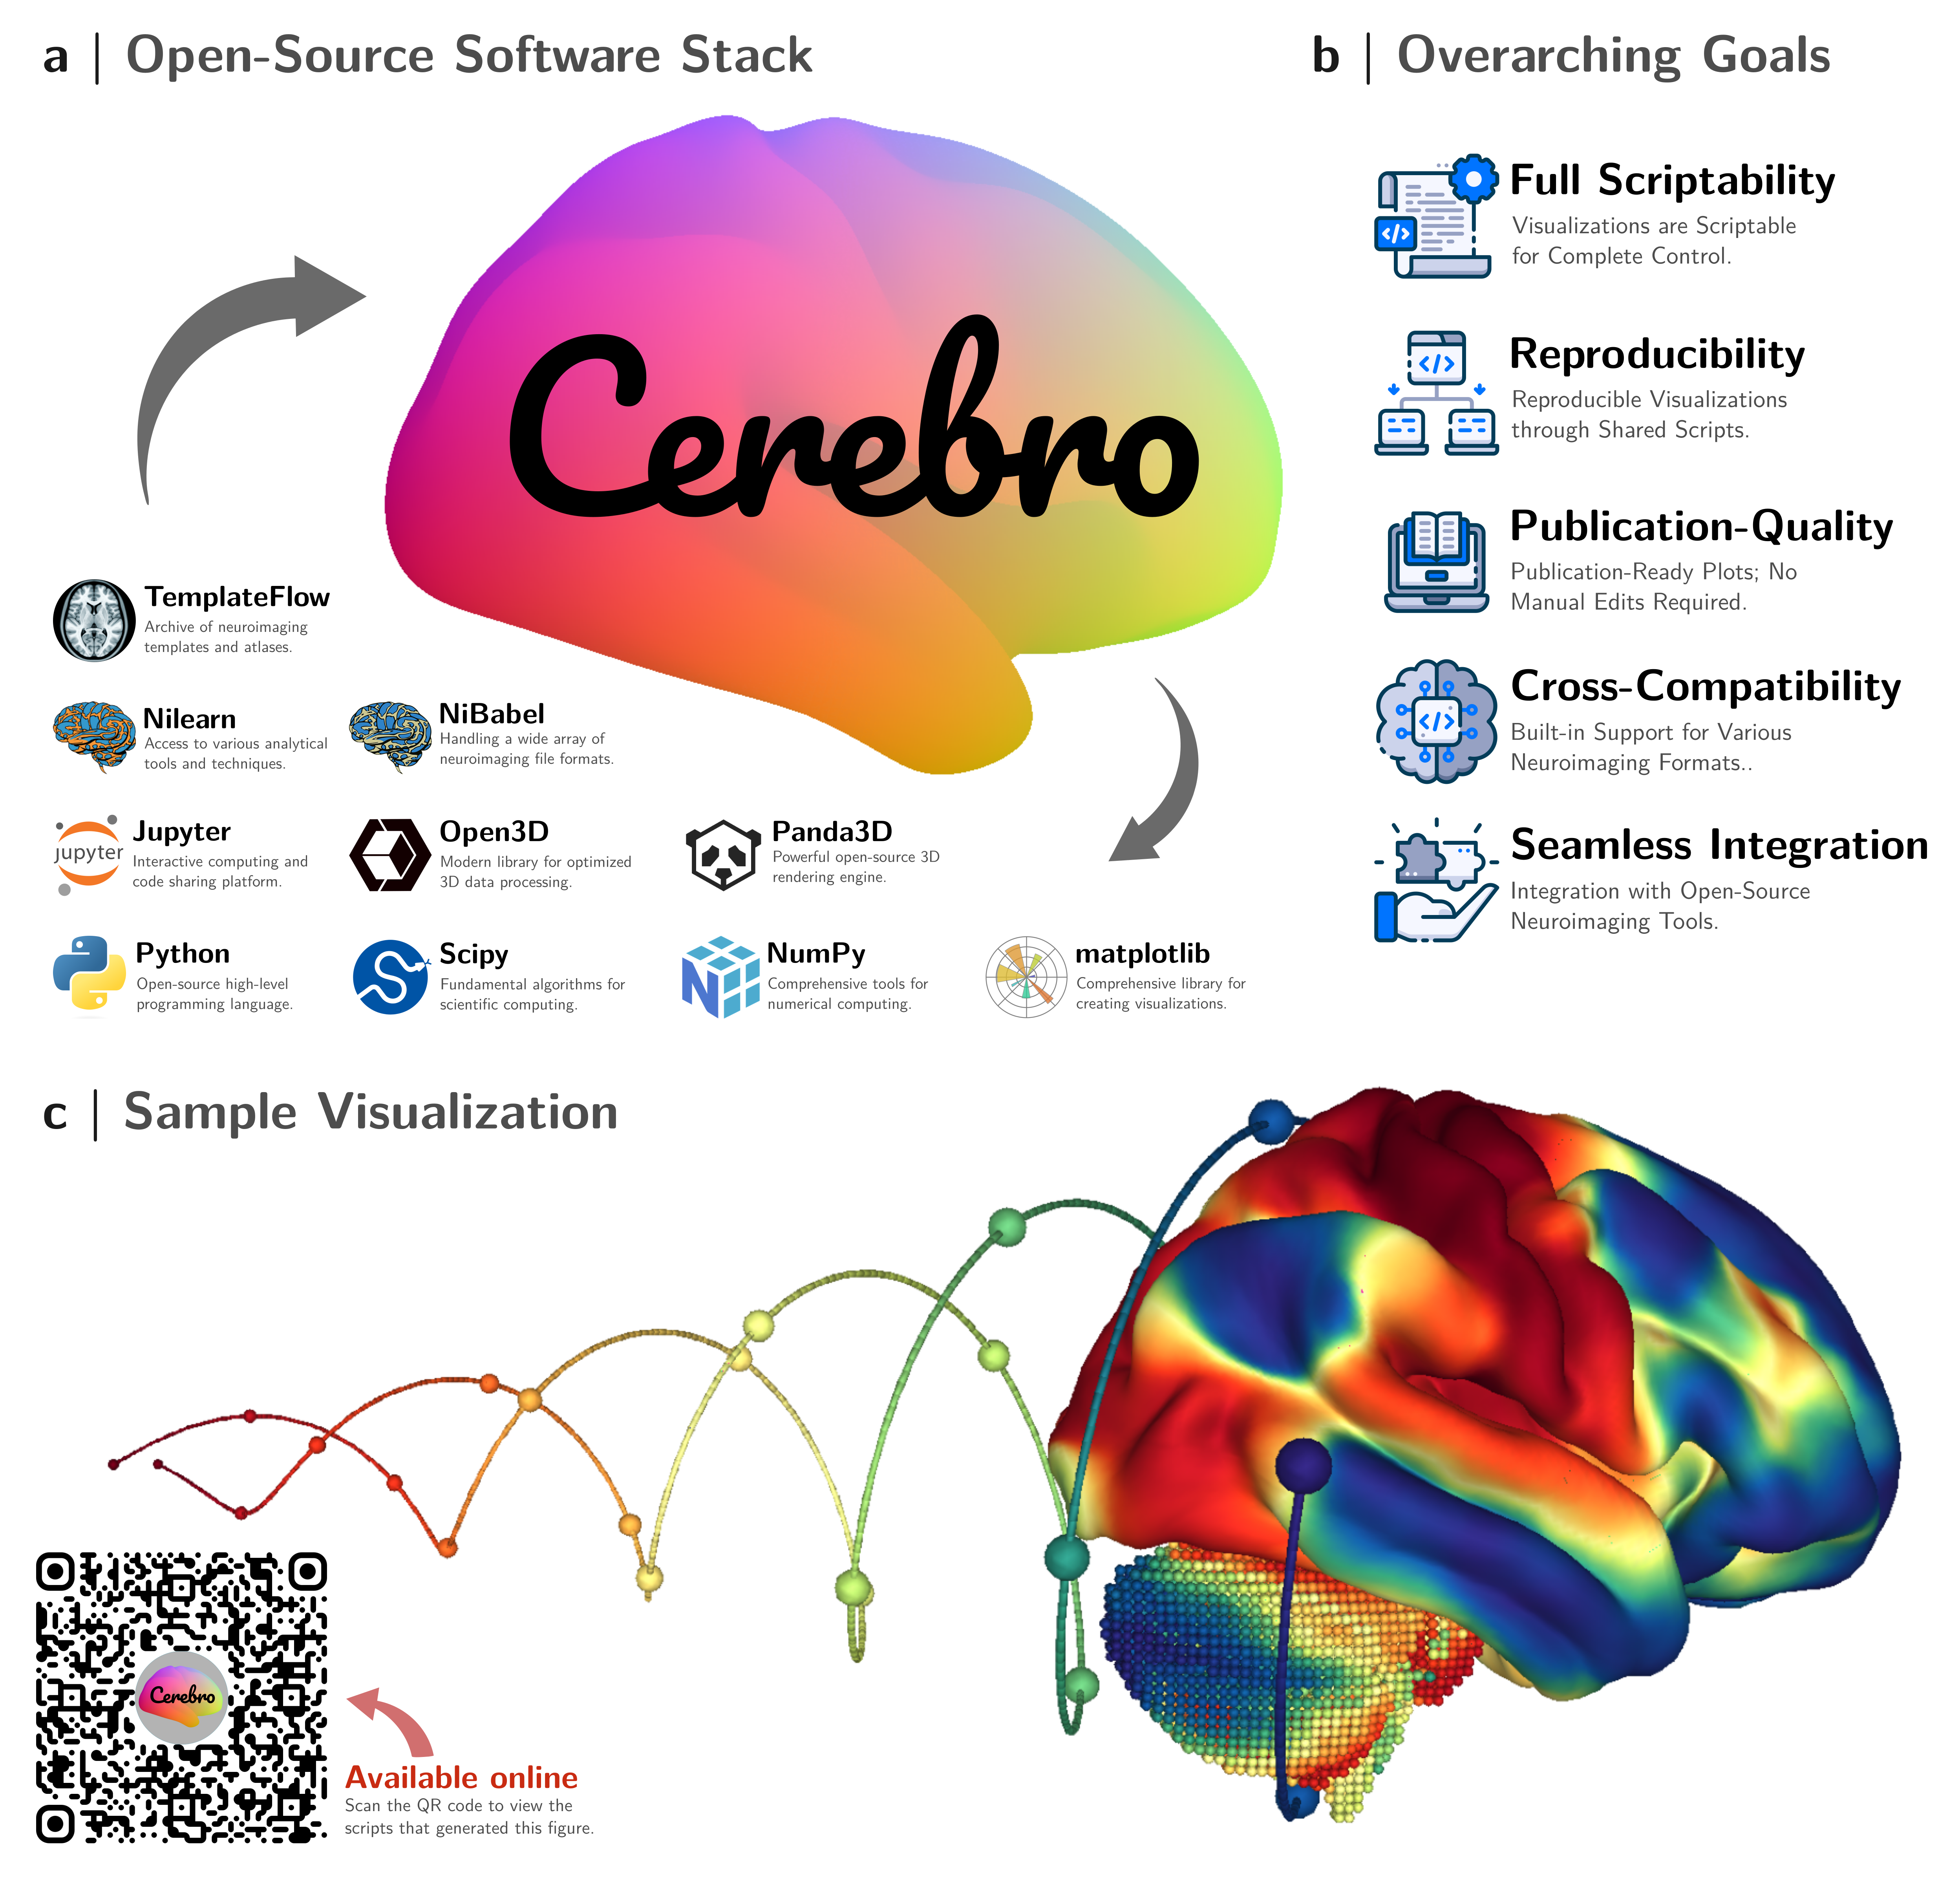
\includegraphics[width=0.8\textwidth]{images/cerebro.png}
    \label{fig:cerebro}
    \caption{
        Cerebro – A Python-Based 3D Brain Visualization Tool. (a) Cerebro leverages an extensive array of open-source Python tools, forming a robust foundation for its functionality. It also integrates with these tools to enable seamless Pythonic neuroimaging visualizations. (b) Cerebro prioritizes principles of scriptability, reproducibility, visualization quality, cross-compatibility, and integration in its pursuit of providing a reliable solution for the neuroimaging community. (c) An illustrative Cerebro-generated visualization, accompanied by a scannable QR code linked to the publicly accessible reproduction scripts.
    }
\end{figure}



\subsection{K-Particles: A visual journey into the heart of magnetic resonance imaging}
\textbf{Authors}: Omer Faruk Gulban, Kenshu Koiso, Thomas Maullin-Sapey, Jeff Mentch, Alessandra Pizzuti, Fernanda Ponce, Kevin R. Sitek, Paul A. Taylor

The primary objective of this project is to leverage particle animations to provide insights into the journey of traveling and sampling the k-space. By generating captivating visualizations, we aim to demystify the concept of k-space and the role it plays in magnetic resonance imaging (MRI), engaging both the scientific community and the general public in a delightful exploration of this fundamental aspect of imaging. This project builds on our previous Brainhack experiences that focused on generating 3D geodesic distance computation animations \cite{Brainhack2021} and particle simulation based brain explosions \cite{Moia2024}.

Our methodology is as follows. First, we start from a 2D brain image (e.g. selecting a slice from a 3D anatomical MRI data
\cite{Brett2023-ia,Numpy,Scipy}. Then, we take its Fourier Transform and subsequently perform masking (or magnitude scaling) operations on k-space data \cite{Bernstein2004}, the transform. We then create simultaneous visualizations of the k-space magnitude and corresponding image-space magnitude data. Note that the masking of k-space data is where the participants of this project exercised their creativity, by setting up various initial conditions and a set of rules to animate the mask data. In the final step, animated frames are compiled into movies to inform (and entertain). The scripts we have used to program these steps are available in \href{https://github.com/ofgulban/k_particles}{GitHub}. Note that, we have also included several animations where no brain images were used, but instead, we generated k-space data directly in k-space to guide the unfamiliar participants with the concepts (see Figure \ref{fig:kparticles}, panel A).

As a result of this hackathon project, a compilation of our progress (see Figure \ref{fig:kparticles}, panel B) can be seen at \href{https://youtu.be/_5ZDctWv5X4}{YouTube} as a video. Some of the highlights are:

\begin{itemize}
\item Audiovisualizer that maps audio features (e.g. amplitude) to k-space mask diameters
\item Game of life \cite{Gardner1970} simulation in k-space with Hermitian symmetry.
\item Pacman moving in k-space is implemented as a series of radial sector masks.
\item Semi-random initialization of particle positions and semi-randomly reassigned velocities that look like an emerging butterfly.
\item Randomized game of life initialization with vanishing trails of the previous simulation steps that look like stars, clouds, and comets orbiting frequency bands in k-space.
\item Semi-random initialization of particle positions and velocities that look like explosions.
\item Predetermined initialization of particle positions (e.g. at the center) and semi-randomized velocities that look like fireworks.
\item Dancing text animations where the positions of text pixels are manipulated by wave functions.
\item Picture based (e.g. cropped faces of the authors) moving within the k space where each pixel’s grayscale value is mapped onto a mask coefficient between 0-1.
\end{itemize}

Our future efforts will involve sophisticating the k-space simulations to generate more entertaining and educational content. For instance, instead of only visualizing the magnitude images, we can generate four panel animations showing real and imaginary (or magnitude and phase) components of the data.

\begin{figure}[hbt!]
    \centering
    \includegraphics[width=0.9\textwidth]{images/k-particles.png}
    \label{fig:kparticles}
    \caption{
        Our compilation of k-space animations generated during the brainhack can be seen at \href{https://youtu.be/XS0LEQExGU8?si=I5Zufp3AcCbdhYIR}{YouTube}.
    }
\end{figure}



\section{Mini-Grant Initiative}

This year, we introduced Mini-Grant initiative, generously supported by sponsors, aimed at empowering and supporting Brainhackers. The grants were distributed across nine categories:
\begin{itemize}
\item Open Science Mini-Grant: Funding projects promoting open science principles like data sharing and open-source software.
\item Diversity and Inclusion Mini-Grant: Supporting initiatives that enhance diversity and inclusion in science or academia.
\item Public Science Communication Mini-Grant: Backing efforts to communicate scientific research to the public in an accessible manner.
\item Innovative Teaching Method Mini-Grant: Encouraging creative approaches to science education.
\item Interdisciplinary Collaboration Mini-Grant: Fostering cross-disciplinary research to address complex challenges.
\item Student-Led Research Mini-Grant: Supporting science projects led by students.
\item Global Science Collaboration Mini-Grant: Encouraging international research collaborations.
\item Early Career Researcher Mini-Grant: Funding early-career scientists to conduct independent projects.
\item Science and Art Integration Mini-Grant: Funding projects that blend scientific concepts with artistic expression.
\end{itemize}

These grants were based on project merit, with nominations made by teams or peers after the project pitches and rhyming battle.
However, the response was less enthusiastic than anticipated, receiving only a limited number of nominations.
This outcome prompted a reflection on the initiative's alignment with the community's core values.
The competitive nature of the grant-awarding process might resonate poorly with the collaborative and inclusive ethos of the Brainhack community.
In light of these reflections, a decision was made to retain the funds for future Brainhack events, with a new approach in mind.
For the next OHBM Hackathon editions, the organizers could initiate the funding process earlier, allowing participants to submit proposals during registration.
This process will enable us to review the needs of the projects in advance and provide support where it's most needed, such as for essential equipment like webcams or help with travel arrangement costs.
The pivotal strategy aims to demonstrate our commitment to the community and ensure that support is available from the outset, fostering a more inclusive and resourceful environment

\section{Rhyming Battle}

One of the most memorable and engaging events at the OHBM Brainhack 2023 was the 'Rhyming Battle.'
Held before the project presentations, this unique event featured three participants who artistically expressed their experiences and challenges encountered during the hackathon.
They crafted short poems about their projects and the various aspects they faced during Brainhack, bringing a touch of lighthearted humour to their scientific endeavours (see Appendix for lyrics).
The Rhyming Battle provided an entertaining break from the Hackathon's more scientific aspects.
It allowed attendees to resonate with each other's experiences, celebrating the struggles and triumphs inherent in scientific projects.
The event showcased the creative and vibrant spirit of the Brainhack community.
Voting for the winner was not straightforward, as the attendees were equally good.
The prize was a single 3D homemade sculpture representing the Brainhack 2023 logo, made for the winner of the battle (Figure \ref{fig:skull}).
However, the enthusiasm of the battlers and the public was overwhelming, and we decided to 3D print the same sculpture for every battle participant.
Ultimately, the spirit of Brainhack community prevailed \cite{gau2021brainhack,levitis2021centering}, and every participant was celebrated as a winner.

\begin{figure}[hbt!]
    \centering
    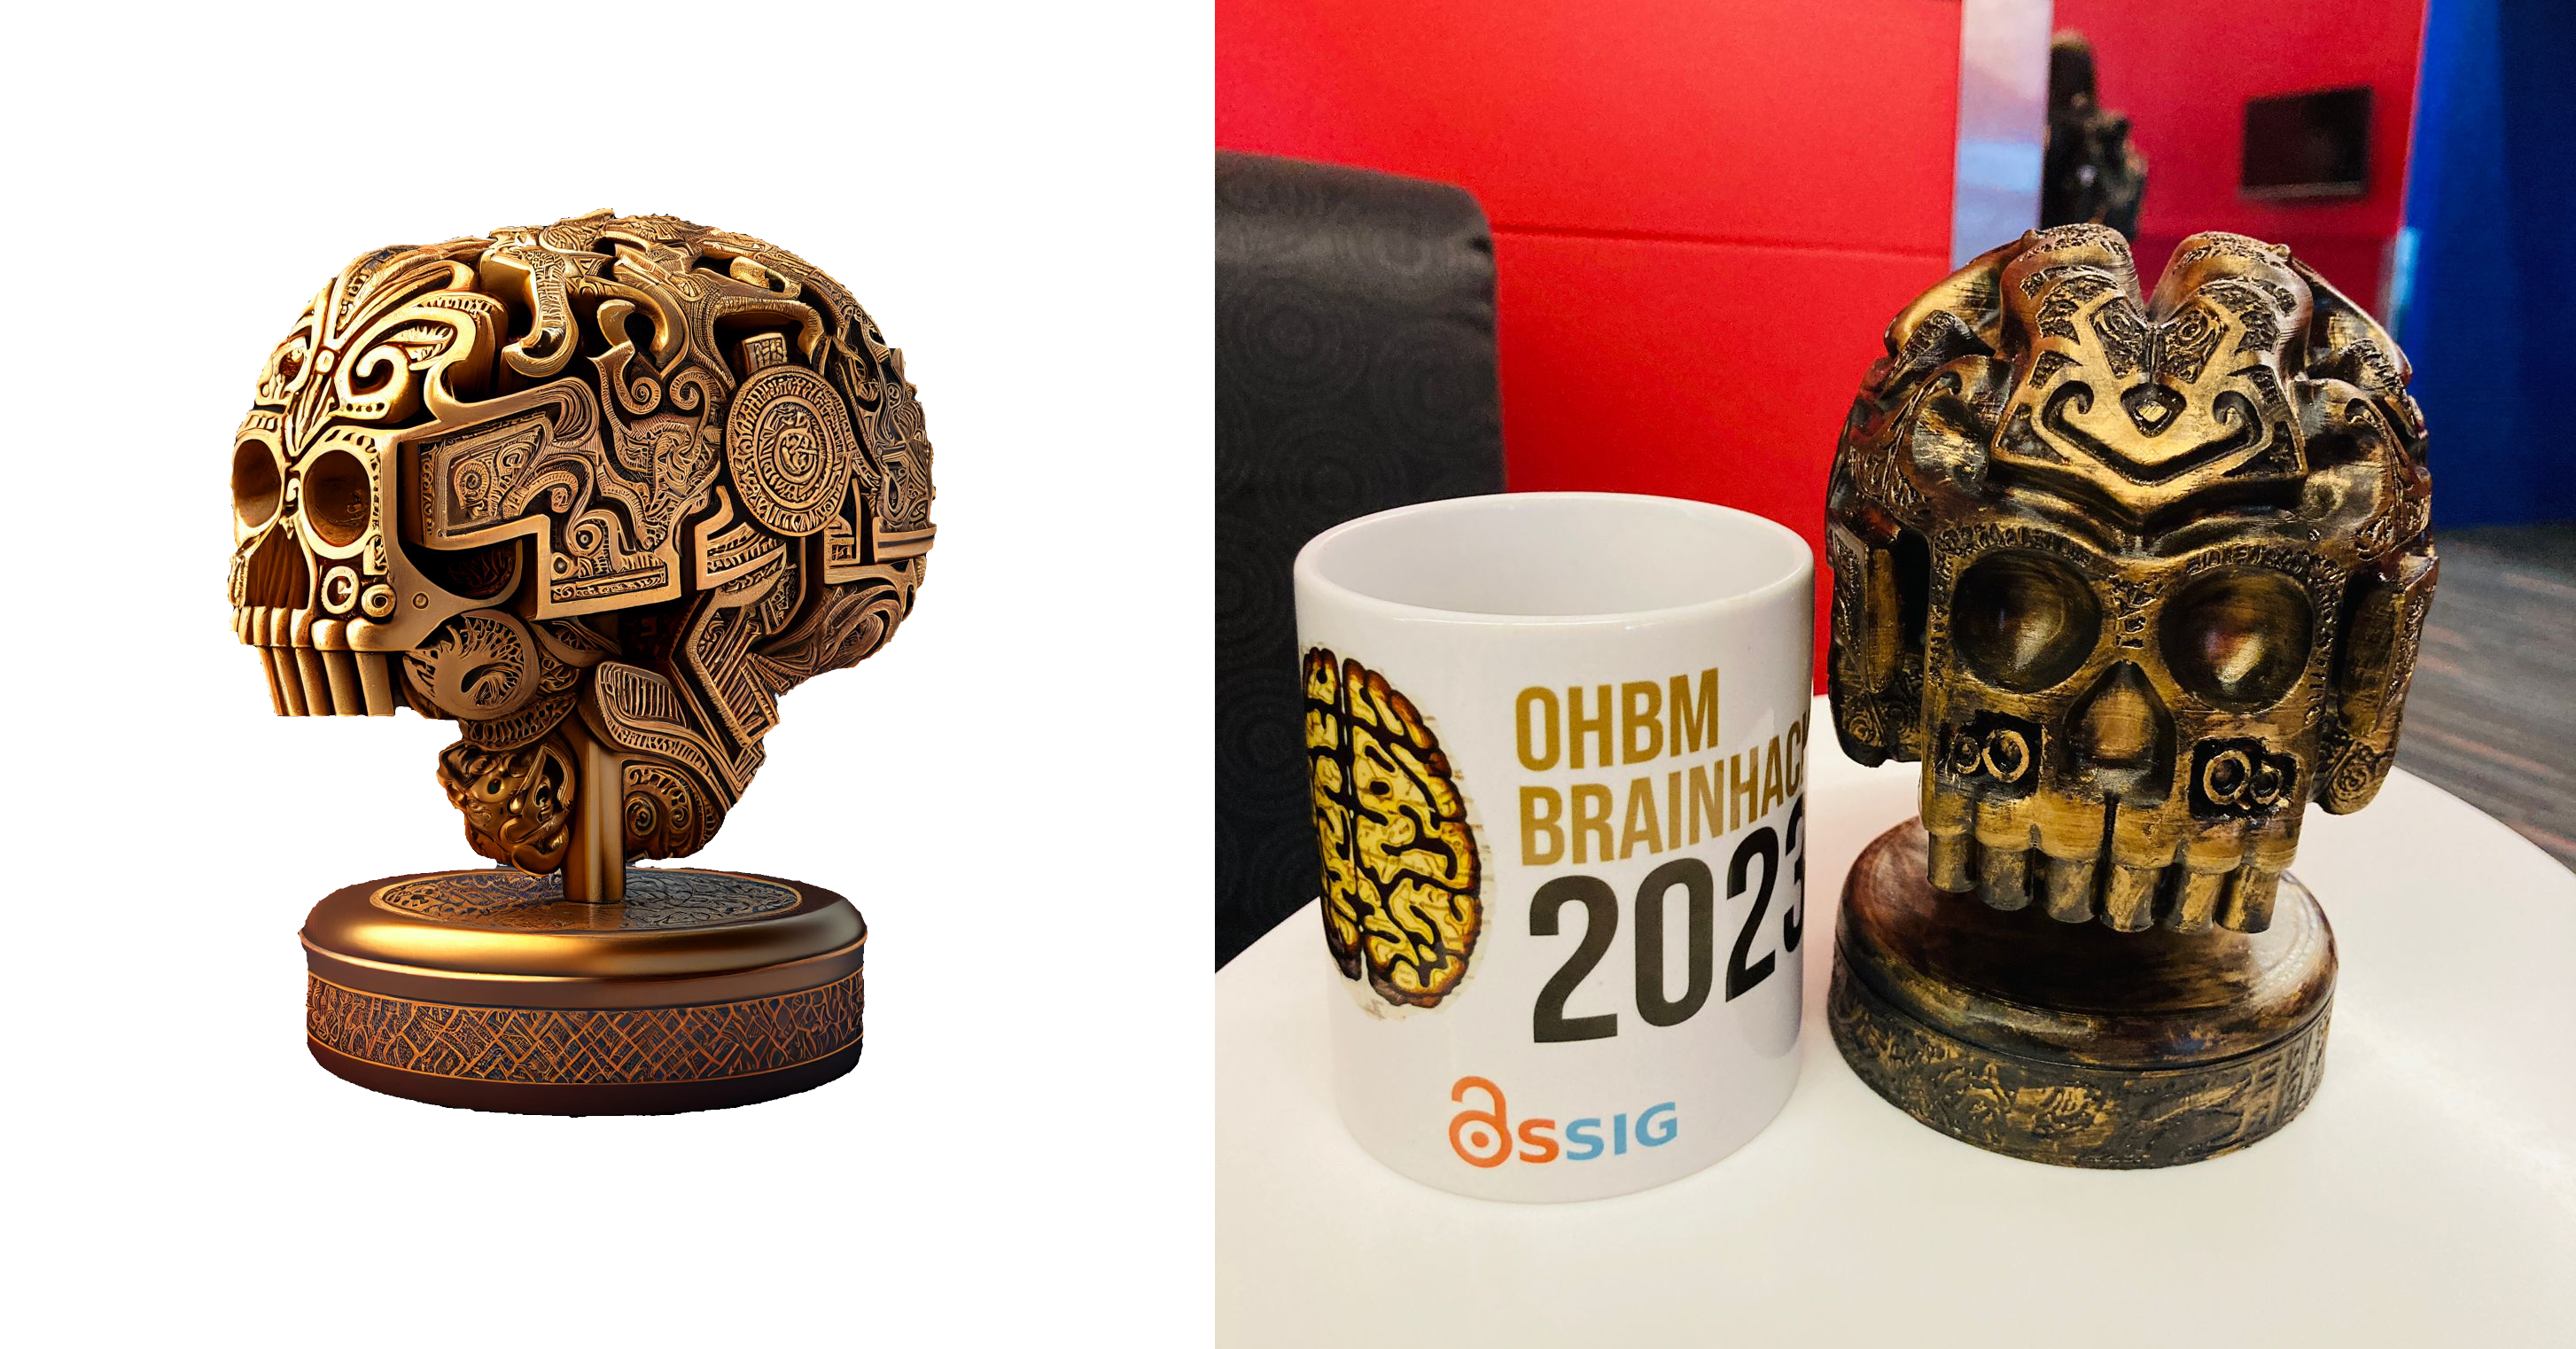
\includegraphics[width=0.9\textwidth]{images/skull.png}
    \label{fig:skull}
    \caption{
        Skull sculpture generated using MidJourney's generative models for the main website and 3D printed replica for the Rhyming Battle winner.
    }
\end{figure}

\section{Conclusion}

The OHBM Brainhack 2023 exemplified a vibrant fusion of education, innovation, and community spirit.
Through initiatives like Train-Track, Hack-Track, the Buddy System, the Rhyming Battle, and the Mini-Grant program, the event fostered an environment rich in learning, creativity, and collaboration.
These elements, coupled with a commitment to open science and diversity, underscored the gathering's success in nurturing a dynamic scientific community.
Reflecting on the experiences and feedback from this year, Brainhack is poised to evolve, embracing lessons learned to enhance future hackathons.
This continuous improvement and deepened community engagement are set to further empower and inspire participants in the years to come.

\bibliographystyle{plain}
\bibliography{refs}

\end{document}
